\newpage
\section{Assembler}

	\lstset{basicstyle=\ttfamily\scriptsize\mdseries}
	
	\begin{multicols}{2}
		\subsection{Binärzahlen}
		{\scriptsize
		\renewcommand{\arraystretch}{1.2}
		\begin{tabular}{r|c|r}
			0 & 0000 & 0 \\
			1 & 0001 & 1 \\
			2 & 0010 & 2 \\
			3 & 0011 & 3 \\
			4 & 0100 & 4 \\
			5 & 0101 & 5 \\
			6 & 0110 & 6 \\
			7 & 0111 & 7 \\
			\nop{0 & 0000 & 0 &    4 & 0100 & 4 &    8 & 1000 & 8 &    12 & 1100 & c \\
			1 & 0001 & 1 &    5 & 0101 & 5 &    9 & 1001 & 9 &    13 & 1101 & d \\
			2 & 0010 & 2 &    6 & 0110 & 6 &   10 & 1010 & a &    14 & 1110 & e \\
			3 & 0011 & 3 &    7 & 0111 & 7 &   11 & 1011 & b &    15 & 1111 & f }
		\end{tabular} \quad
		\begin{tabular}{r|c|r}
			 8 & 1000 & 8 \\
			 9 & 1001 & 9 \\
			10 & 1010 & a \\
			11 & 1011 & b \\
			12 & 1100 & c \\
			13 & 1101 & d \\
			14 & 1110 & e \\
			15 & 1111 & f 
		\end{tabular} \qquad
		\begin{tabular}{r @{ = } l}
			$2^{0}$ & 1 \\
			$2^{1}$ & 2 \\
			$2^{2}$ & 4 \\
			$2^{3}$ & 8 \\
			$2^{4}$ & 16 \\
			$2^{5}$ & 32 \\
			$2^{6}$ & 64 \\
			$2^{7}$ & 128
		\end{tabular} \quad
		\begin{tabular}{r @{ = } l}
			$2^{8}$ & 256 \\
			$2^{9}$ & 512 \\
			$2^{10}$ & 1024 \\
			$2^{11}$ & 2048 \\
			$2^{12}$ & 4096 \\
			$2^{13}$ & 8192 \\
			$2^{14}$ & 16384 \\
			$2^{15}$ & 32768
		\end{tabular}
		}
		
	\end{multicols}
	
	\subsection{Instructions}
		a = b + c\tab	add a, b, c\\
		a = b - c\tab	sub a, b, c\\
		\$s0-\$s7 \tab \$t0-\$t9\tab are memory in the SPRAM register, t are temporary(local) and s are saved.
		\begin{center}
				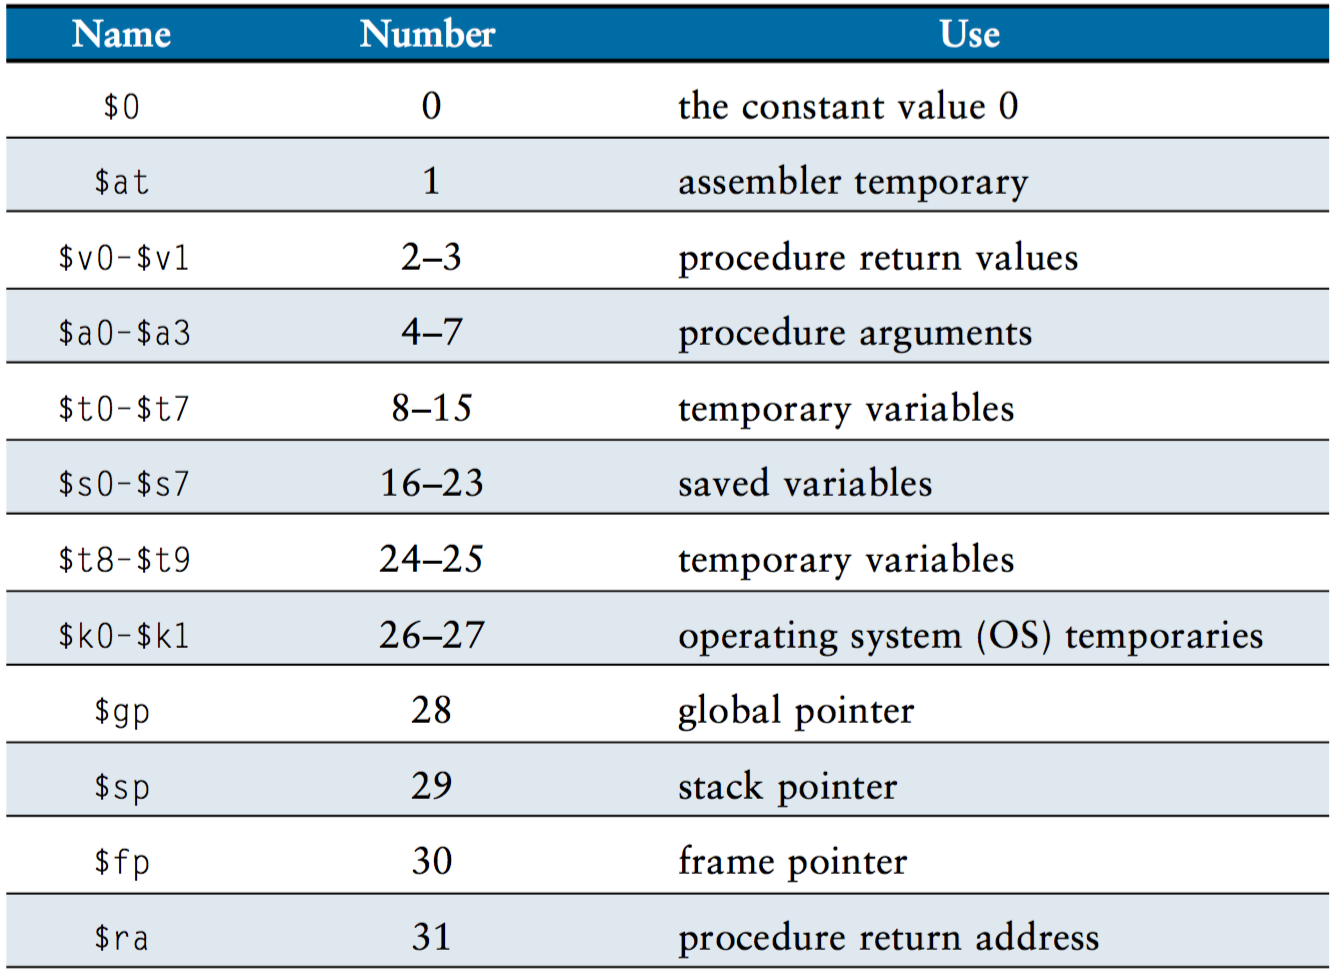
\includegraphics[width = 9cm]{images/reg}
		\end{center}
		lw \$s3, 1(\$0)\tab \#load memory word (0+1 = 1) into s3\\
		sw \$s3, 3(\$0)\tab \#write s3 into memory word 3\\
		\begin{center}
				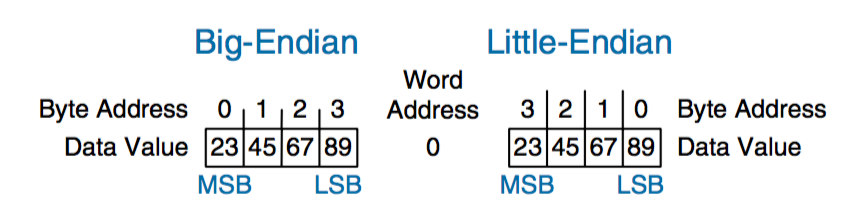
\includegraphics[width = 9cm]{images/big}
		\end{center}
		Each word in memory consists of 4 bytes, therefore you have to store in memory by a multiple of 4.\\
		addi \$s1, \$s0, -12\tab you use addi to add constants to two  register operands, there is no subi so use negative numbers instead.\\
		You can use addi to initialise a constant ex\tab addi \$s0, \$0, ox4f3c\tab initialisis \$s0 to ox4f3c
		\subsubsection{Intructions types}
		There are three instruction types R-type, I-type, and J-type. R-type instructions operate on three registers(add, sub). I-type instructions operate on two registers and a 16-bit immediate(addi,lw, sw). J-type (jump) instructions operate on one 26-bit immediate.\\Each instruction is stored in a 32 bit word. So a program consists of 32 bit numbers representing the instructions.
		\subsubsection{Logic instructions}
		R-type:\\ and s1, s2, s3\tab writes two s1 the bytes that are both 1 in s2 and s3\\
		there is also or and nor\\
		I-type: andi, ori and xori\tab they work the same as R-type but put a fix value in hexadecimal instead of last operand.
		\subsubsection{Shifts}
		Are R-type: sll(v) shift left logical, srl(v) shift right logical and sra(v) shift right arithmetic. Shifting a value left by n is like multiplying it with $2^n$. shifting a value right by n is like dividing it with $2^n$. arithmetic shifts and places one's instead of zeros.
		\subsubsection{mult in div}
		mult \$s0, \$s1\tab multiplies s0 with s1 the 32 most significant bits are placed in hi and 32 least in lo.\\
		div \$s0, \$s1\tab the qoutient is placed in lo and the remainder in hi
		\subsubsection{branching}
		if else is executed with branching and beq(branch if equal) and bne(branch if not equal) instructions.
		\begin{center}
				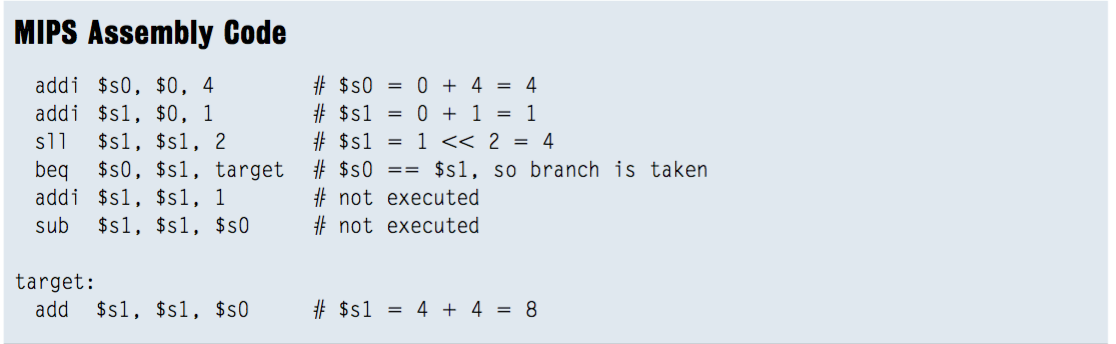
\includegraphics[width = 18cm]{images/beq}
		\end{center}
		\begin{center}
				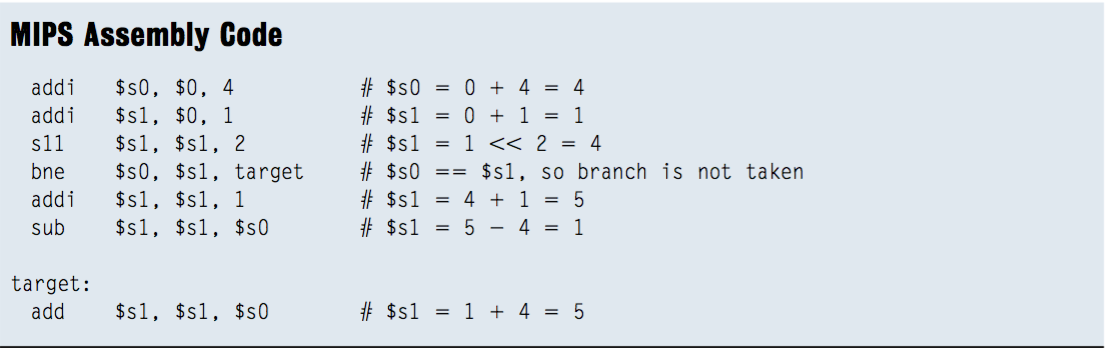
\includegraphics[width = 18cm]{images/bne}
		\end{center}
		If it's true it executes the target, else it executes the code after and then the targer.
		\subsubsection{jump}
			There are 3 jump instruction j, jr and jal. j just jumps to the specified label ex\\
			j\tab target\tab jumps to targer\\
			jr jumps to the address held in a register and jal is similar to j but is used by procedures to save a return address.
		\subsubsection{if else case}
		You can make if else statements using beq and bne:
		\begin{center}
				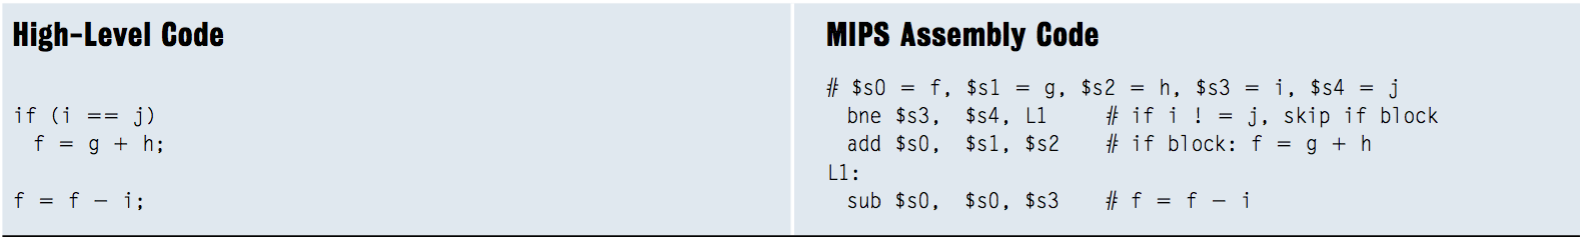
\includegraphics[width = 18cm]{images/if}
		\end{center}
		\begin{center}
				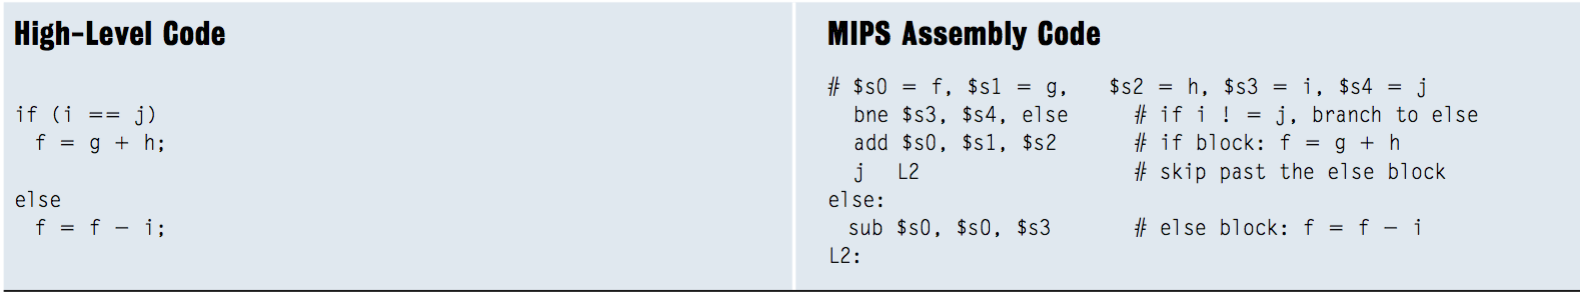
\includegraphics[width = 18cm]{images/else}
		\end{center}
		You can implement a case by using multiple if else statements.
		\begin{center}
				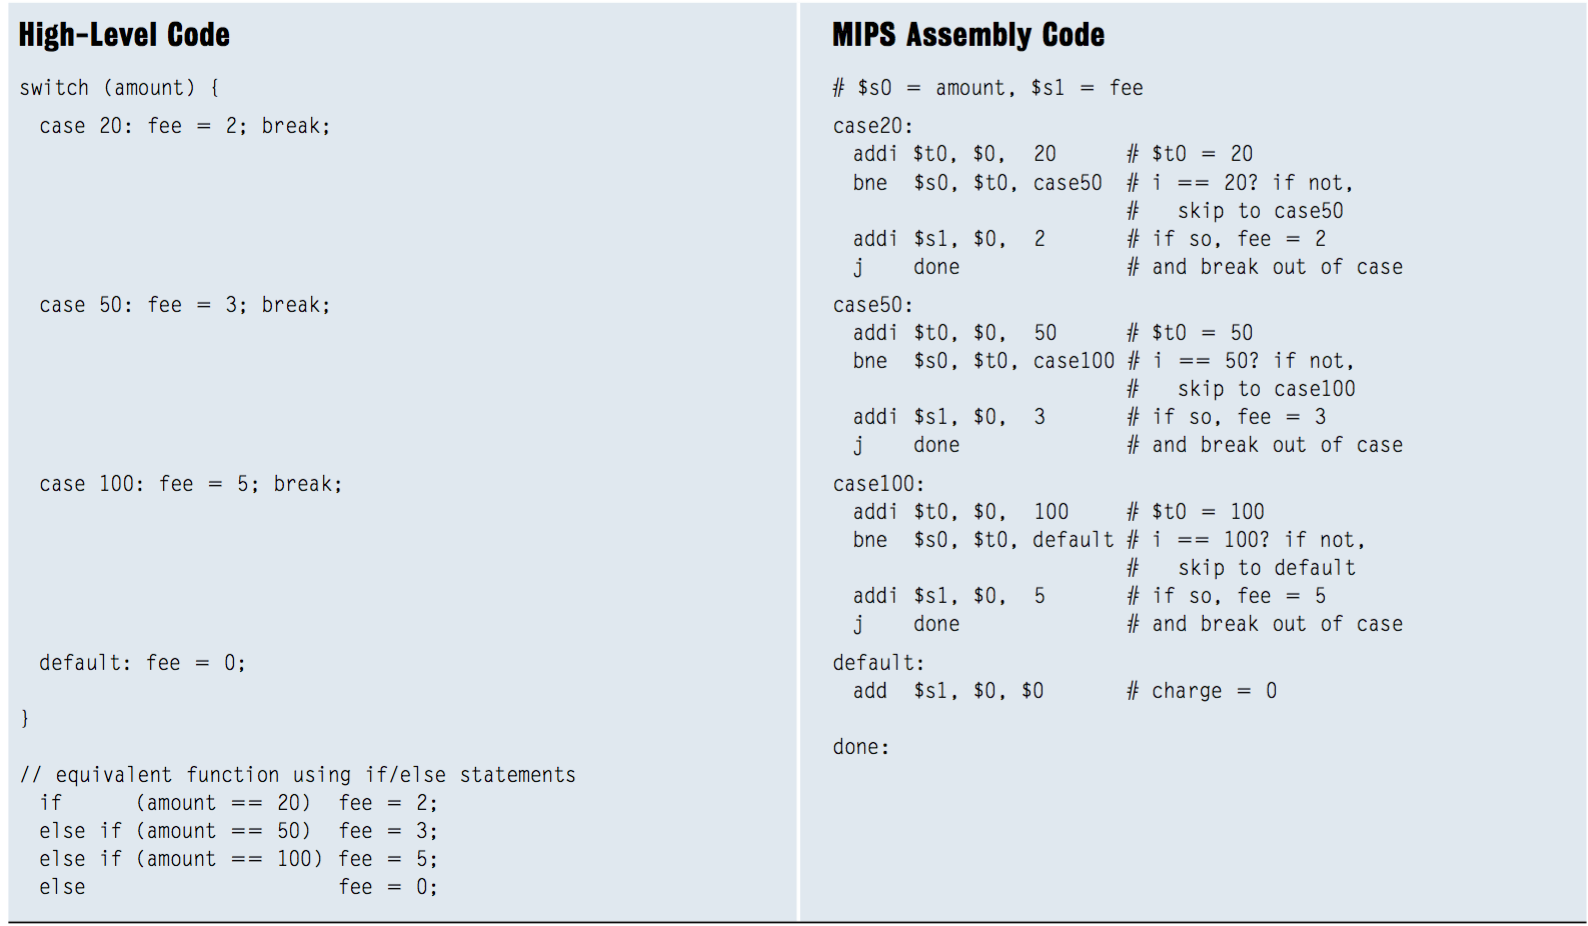
\includegraphics[width = 18cm]{images/case}
		\end{center}
		\subsubsection{Loops}
		For loops you can use the same principal as for the case but if a condition is met it will skip to the same section.
		\begin{center}
				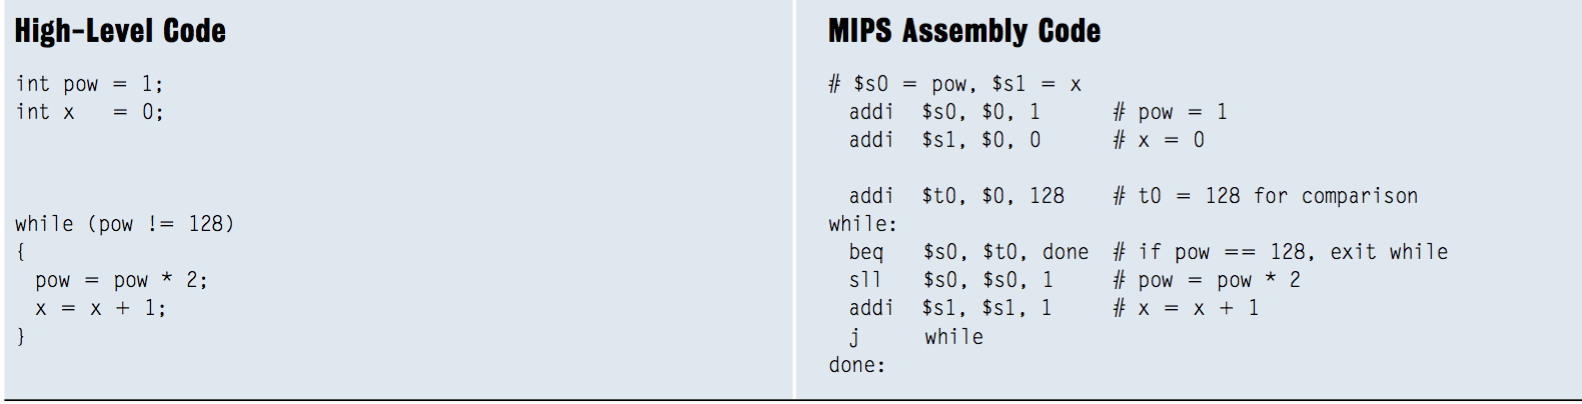
\includegraphics[width = 18cm]{images/while}
		\end{center}
		\begin{center}
				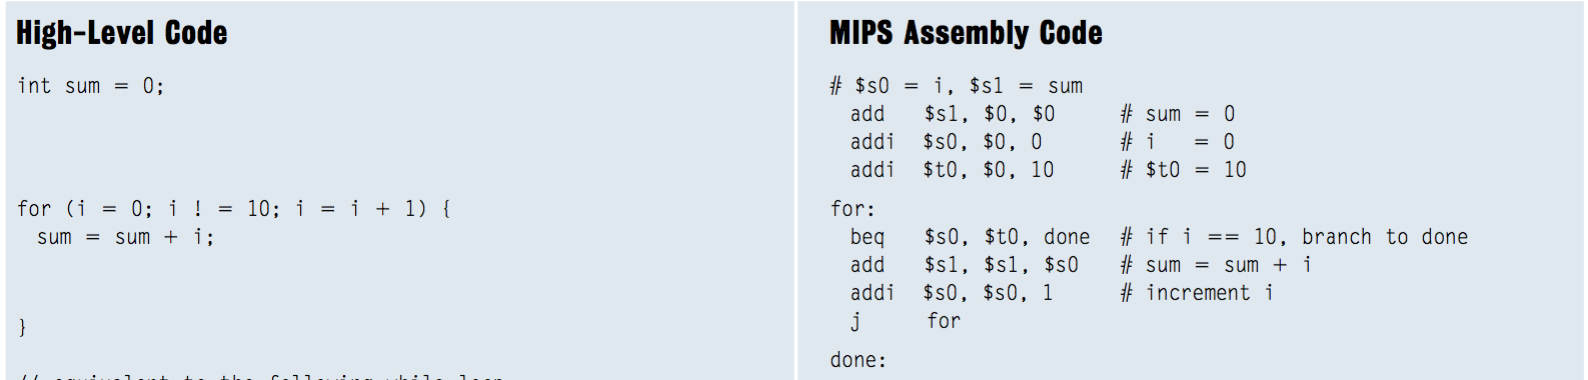
\includegraphics[width = 18cm]{images/for}
		\end{center}
		\subsubsection{magnitude comparison}
		To use a smaller than:\\
		slt rd, rs, rt\tab sets rd to 1 when rs < rt. Otherwise, rd is 0.
		\subsubsection{Arrays}
		A array is basically a address in memory which you increment by 4 to reach the other array values.
		\begin{center}
				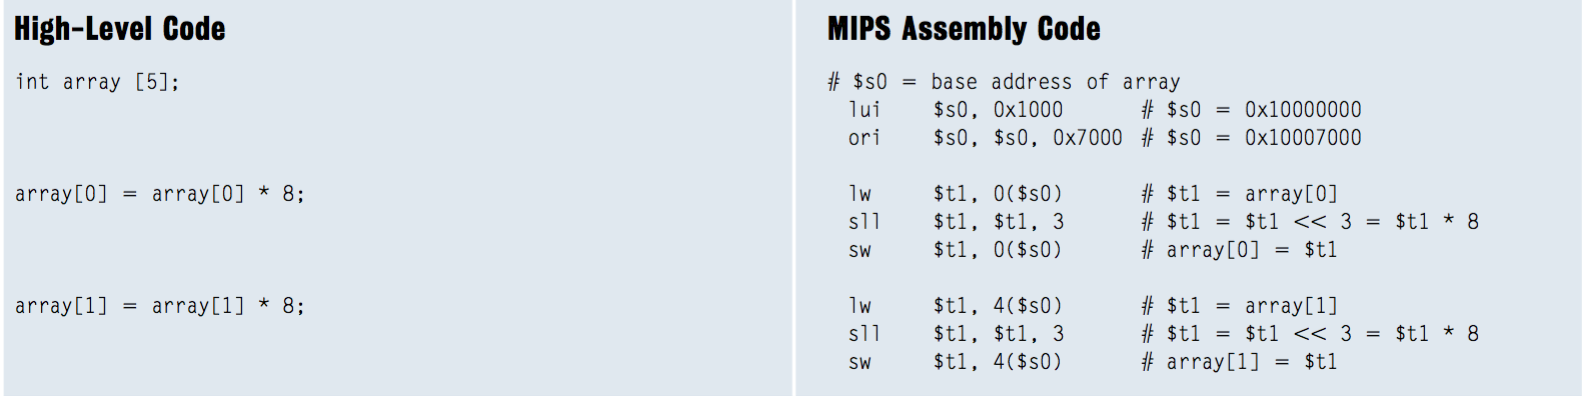
\includegraphics[width = 18cm]{images/array}
		\end{center}
		\subsubsection{Functions}
		To call a procedure jal is used and jr \$ra(ra saves the address for where it should jump to after the loop) is used to return from a procedure. Procedures use \$a0-\$a3 as input arguments and \$v0-\$v1 as return values.
		\begin{center}
				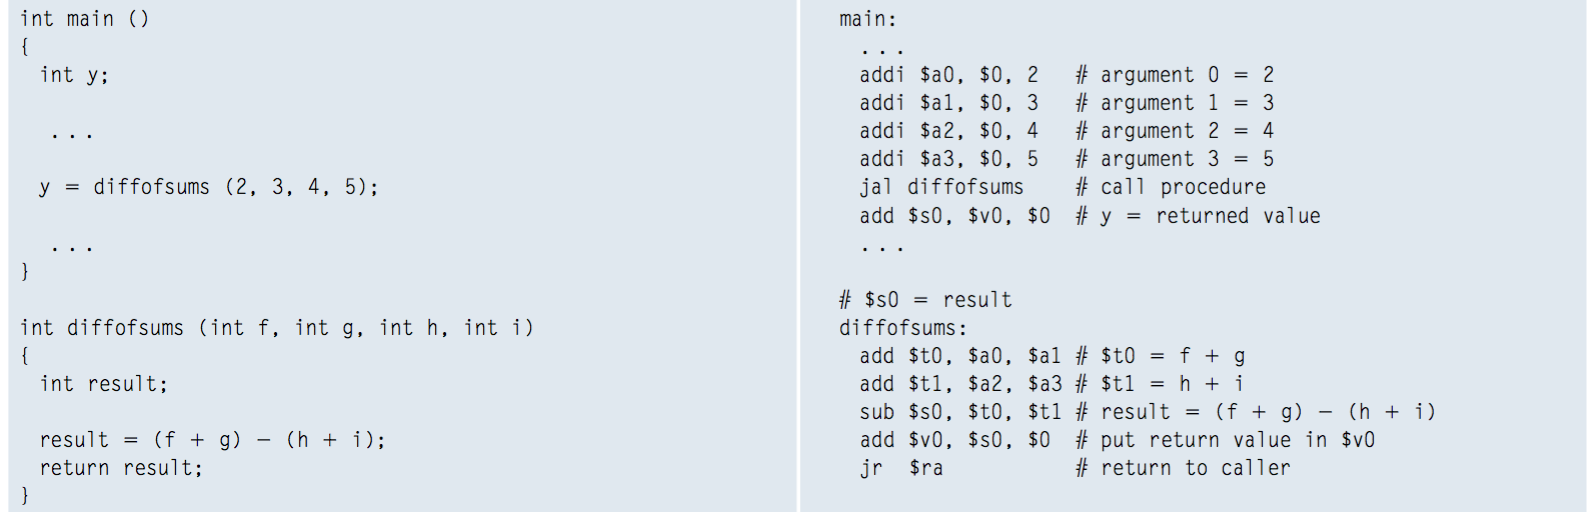
\includegraphics[width = 18cm]{images/function}
		\end{center}
		The implementation of diffofsums is not great because it changes the value of s0 which it shouldn't. To ameliorate this diffofsums should only use t variables or restore the value of s0 after the function using a stack.
		\subsubsection{stacks}
		Stacks are a LIFO queue. Better version of diffofsums using a stack:
		\begin{center}
				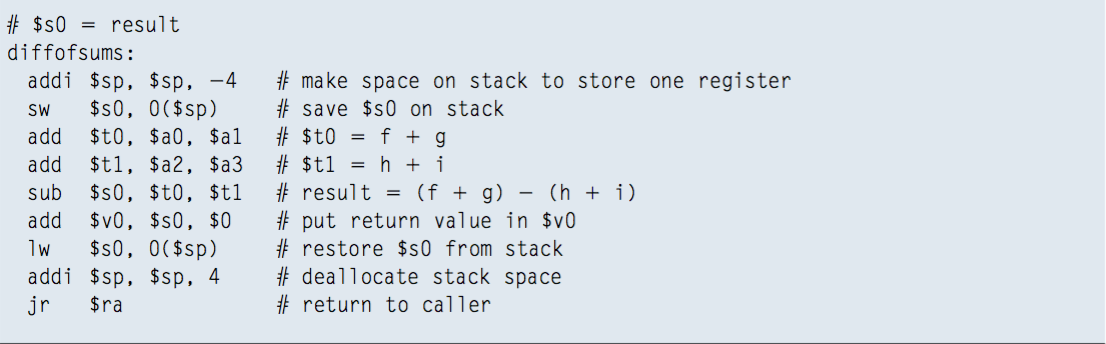
\includegraphics[width = 18cm]{images/stack}
		\end{center}
		\begin{center}
				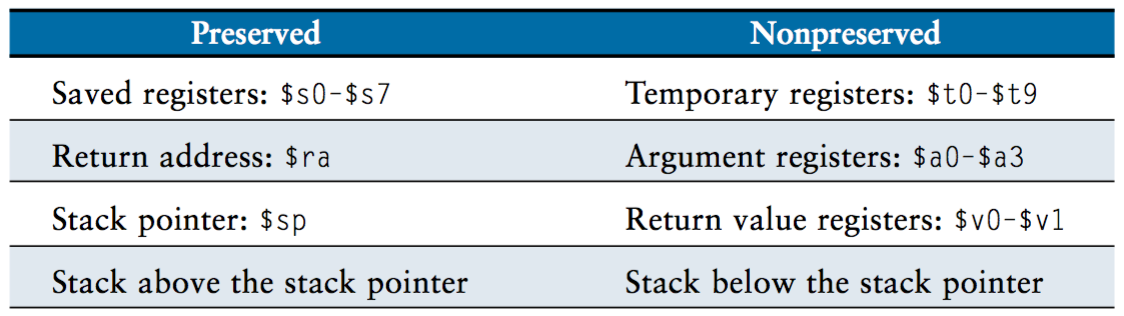
\includegraphics[width = 9cm]{images/preserved}
		\end{center}
		In recursive function calls you have to restore also non preserved registers.\\
		If more than 4 input variables are needed you can use the stack.\\
		global variables are \$gp
		\subsubsection{the Program just for interest}
		\begin{center}
				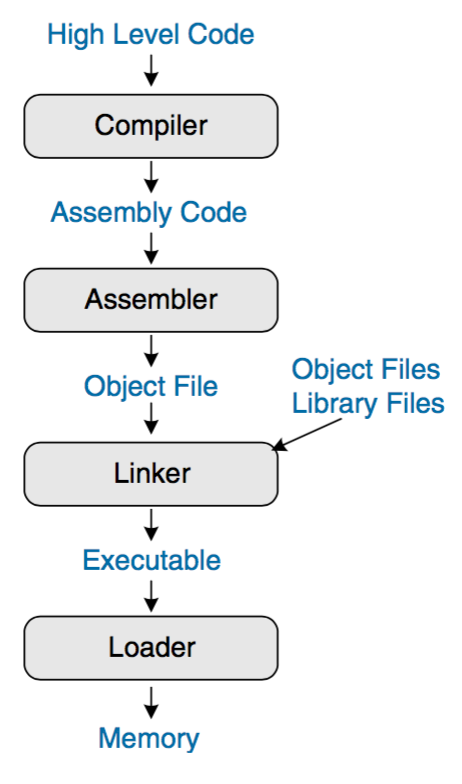
\includegraphics[height = 9cm]{images/program}
		\end{center}
		

